\documentclass{article}
\usepackage{graphicx}
\usepackage{amsmath}
\usepackage{enumitem}
\usepackage{float}
\usepackage{listings}
\usepackage{xcolor}
\usepackage{caption}
\usepackage[a4paper, margin=1in]{geometry}

% Custom information
\newcommand{\className}{Course: Automatic Control Systems – ASEN 5114-001 – Spring 2025}
\newcommand{\professorName}{Professor: Dale Lawrence}
\newcommand{\taName}{Teaching Assistant: Anantha Dhruva}
\title{Homework 3 \\ \className \\ \professorName \\ \taName}
\author{Steve Gillet}
\date{\today}

\lstdefinestyle{matlabstyle}{
    language=Matlab,              % Specify the language
    basicstyle=\ttfamily\footnotesize\color{black}, % Code font
    keywordstyle=\color{blue}\bfseries, % Keywords in blue
    stringstyle=\color{orange},    % Strings in green
    commentstyle=\color{magenta}, % Comments in magenta
    numbers=left,                 % Line numbers on the left
    numberstyle=\tiny\color{black},% Line number style
    stepnumber=1,                 % Line number increment
    breaklines=true,              % Line breaking
    frame=single,                 % Border around code
    backgroundcolor=\color{white},
    tabsize=4,                    % Tab size
    showstringspaces=false,       % Don't show spaces in strings
}

\renewcommand{\thesection}{\arabic{section})}
\renewcommand{\thesubsection}{\arabic{section}.\arabic{subsection}}

\begin{document}

\maketitle
\textit{
    "This provides some practice using the direct state space modeling approach discussed in class.
    Please use this method to work the following problems from the textbook. Undergraduates
    (4114) do problems 1) and 2). Graduate students (5114) do all three problems."
}

\section{}

\textit{
    "Problem 2.5. Develop the state space equations of motion for the car suspension of
    Example 2.2, and simulate the response using the parameters provided in the problem
    statement."
}

Problem 2.5 statement from the textbook:

\textit{
    "2.5. For the car suspension discussed in Example 2.2 , plot the position of the car and the wheel after the car hits a “unit bump” (that is,  is a unit step) using Matlab. Assume 
    $m_1 = 10 kg$, $m_2 = 350 kg$, $K_w = 500,000 N/m$, and $K_s = 10,000 N/m$.
    Find the value of b that you would prefer if you were a passenger in the car."
}

Example 2.2 statement:

\textit{
    "Figure 2.4 shows an automobile suspension system. Write the equations of motion for the automobile and wheel motion assuming one-dimensional vertical motion of one quarter of the car mass above one wheel. A system consisting of one of the four-wheel suspensions is usually referred to as a quarter-car model. The system can be approximated by the simplified system shown in Fig. 2.5 where two spring constants and a damping coefficient are defined. Assume the model is for a car with a mass of 1580 kg, including the four wheels, which have a mass of 20 kg each. By placing a known weight (an author) directly over a wheel and measuring the car’s deflection, we find that 
    $k_s = 130,000 N/m$. Measuring the wheel’s deflection for the same applied weight, we find that 
    $k_w \approx 1,000,000 N/m$. By using the step response data in Fig. 3.19 (b) and qualitatively observing that the car’s response to a step change matches the damping coefficient curve for  in the figure, we conclude that ."
}

\begin{figure}[H]
    \centering
    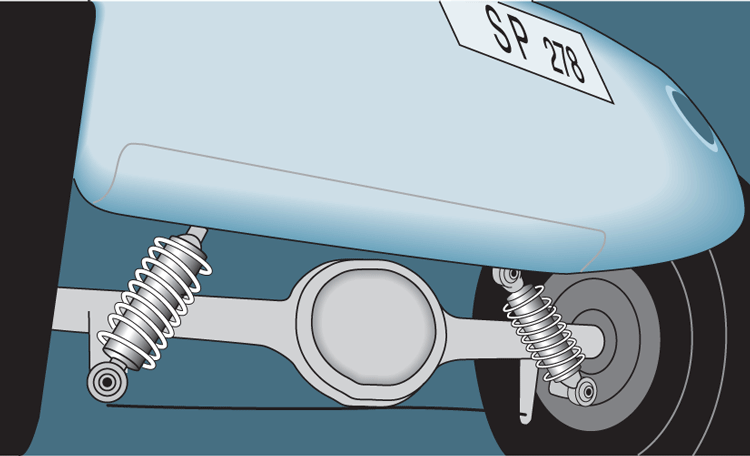
\includegraphics[width=0.5\textwidth]{fig24.png}
    \caption*{Figure 2.4: Automobile suspension}
\end{figure}

\begin{figure}[H]
    \centering
    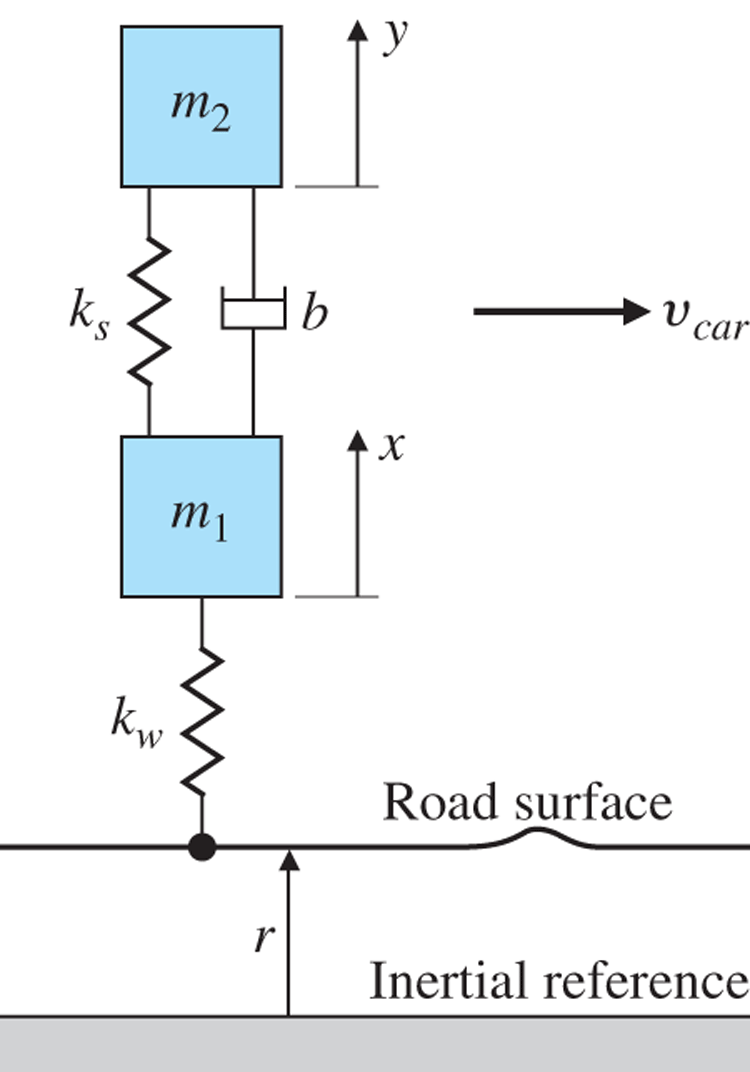
\includegraphics[width=0.5\textwidth]{fig25.png}
    \caption*{Figure 2.5: The quarter-car model}
\end{figure}

\begin{figure}[H]
    \centering
    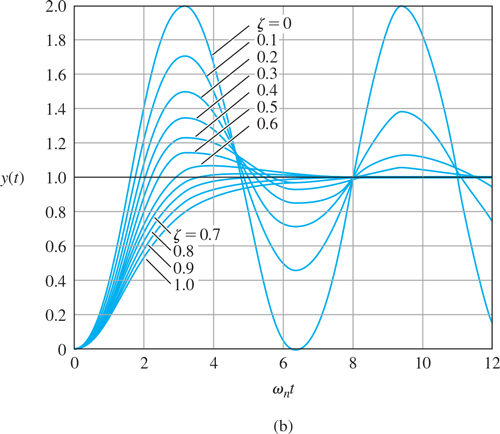
\includegraphics[width=0.5\textwidth]{fig319b.png}
    \caption*{Figure 3.19 (b): Responses of second-order systems versus $\zeta$: step responses}
\end{figure}

\subsection{Identify}
\subsubsection{Input}
\begin{align*}
\text{Input: } & u = r
\end{align*}

\subsubsection{Output}
\begin{align*}
\text{Output: } & y = y \ (\text{or } \ddot{y})
\end{align*}

\subsubsection{States}
\begin{align*}
\text{Mass 2: } & x_1 = v_{m_2} = \dot{y} \\
\text{Spring K: } & x_2 = f_{k_s} \\
\text{Mass 1: } & x_3 = v_{m_1} \\
\text{Spring K: } & x_4 = f_{k_w}
\end{align*}

\subsection{Canonical State Variables}
\begin{align*}
x^*_1 &= f_{m_2}, \quad x^*_2 = v_{k_s}, \quad x^*_3 = f_{m_1}, \quad x^*_4 = v_{k_w}
\end{align*}

\subsection{Topology Equations}
\begin{align*}
x^*_1 &= f_{m_2} = -f_{k_s} - f_b = -f_{k_s} - bv_b = -f_{k_s} - b(v_{m_2} - v_{m_1}) = -x_2 - b(x_1 - x_3) \\
x^*_2 &= v_{k_s} = v_{m_2} - v_{m_1} = x_1 - x_3 \\
x^*_3 &= f_{m_1} = -f_{k_w} + f_{k_s} + f_b = -x_4 + x_2 + b(x_1 - x_3)\\
x^*_4 &= v_{k_w} = v_{m_1} - \dot{r} = x_3 - \dot{r}
\end{align*}

\subsection{Energy Storage Element Equations}
\begin{align*}
x^*_1 &= f_{m_2} = m_2 \dot{v}_{m_2} = m_2 \dot{x}_1 \Rightarrow \dot{x}_1 = \frac{1}{m_2} (x_1^*) = \frac{1}{m_2} (-x_2 - b(x_1-x_3)) \\
x^*_2 &= v_{k_s} = \frac{1}{k_s} \dot{f}_{k_s} = \frac{1}{k_s} \dot{x}_2 \Rightarrow \dot{x}_2 = k_s x^*_2 = k_s (x_1 - x_3) \\
x^*_3 &= f_{m_1} = m_1 \dot{v}_{m_1} = m_1 \dot{x}_3 \Rightarrow \dot{x}_3 = \frac{1}{m_1} (x_3^*) = \frac{1}{m_1} (-x_4 + x_2 + b(x_1 - x_3)) \\
x^*_4 &= v_{k_w} = \frac{1}{k_w} \dot{f}_{k_w} = \frac{1}{k_w} \dot{x}_4 \Rightarrow \dot{x}_4 = k_w(x^*_4) = k_w (x_3 - \dot{r})
\end{align*}

\subsection{Collect in Matrix Form}
\[
\begin{bmatrix}
\dot{x}_1 \\
\dot{x}_2 \\
\dot{x}_3 \\
\dot{x}_4
\end{bmatrix}
=
\begin{bmatrix}
-\frac{b}{m_2} & -\frac{1}{m_2} & \frac{b}{m_2} & 0 \\
k_s & 0 & -k_s & 0 \\
\frac{b}{m_1} & \frac{1}{m_1} & -\frac{b}{m_1} & -\frac{1}{m_1} \\
0 & 0 & k_w & 0
\end{bmatrix}
\begin{bmatrix}
x_1 \\
x_2 \\
x_3 \\
x_4
\end{bmatrix}
+
\begin{bmatrix}
0 \\
0 \\
0 \\
-k_w
\end{bmatrix}
\dot{r}
\]

\[
y = 
\begin{bmatrix}
1 & 0 & 0 & 0
\end{bmatrix}
\begin{bmatrix}
x_1 \\
x_2 \\
x_3 \\
x_4
\end{bmatrix}
+
\begin{bmatrix}
0
\end{bmatrix}
u
\]

\subsection*{Simulation}

After deriving the state space model for the system I put that model into Matlab using the 'ss' function and the parameters from the Problem 2.5 statement.
The problem statement asks to find a suitable b value, so I started with 1.

\begin{lstlisting}[style=matlabstyle]
b = 1;
m1 = 10; % [kg]
m2 = 350; % [kg]
kw = 500000; % [Nm]
ks = 10000; % [Nm]


A = [-b/m2 -1/m2 b/m2 0; ks 0 -ks 0; 0 0 0 -1/m1; 0 0 kw 0]; 
B = [0; 0; 0; -kw];       
C = [1 0 0 0];        
D = [0];  

carSusSS = ss(A, B, C, D);
carSusTF = tf(carSusSS);
disp(carSusTF);
\end{lstlisting}

Then I got the transfer function from that state space model using the 'tf' function in Matlab and passed that to a simulink model to simulate.
Then I built the system in simulink using a step input and a continuous transfer function block.

\begin{figure}[H]
    \centering
    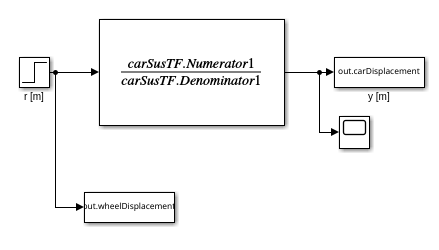
\includegraphics[width=0.75\textwidth]{carSusSimModel.png}
\end{figure}

Then I ran the simulation at $b=1$ and you can see that there basically is no damping and the system just kind of bangs up and down.

\begin{figure}[H]
    \centering
    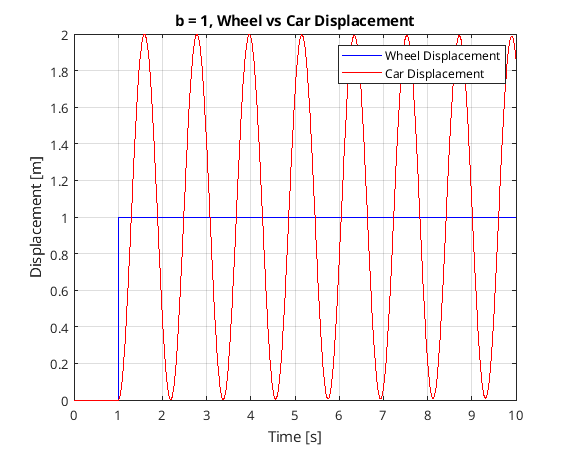
\includegraphics[width=0.75\textwidth]{b1sim.png}
\end{figure}

Then I tried a few different values for b until I worked my way up to 100 where you can start to see some damping take effect.

\begin{figure}[H]
    \centering
    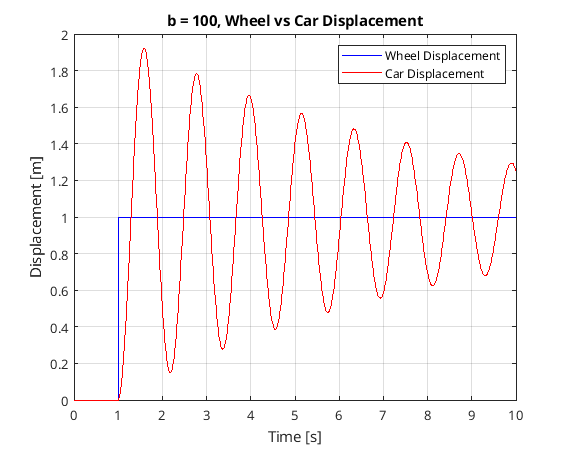
\includegraphics[width=0.75\textwidth]{b100sim.png}
\end{figure}

At b 1,000 I finally saw some behavior that looked pretty good.

\begin{figure}[H]
    \centering
    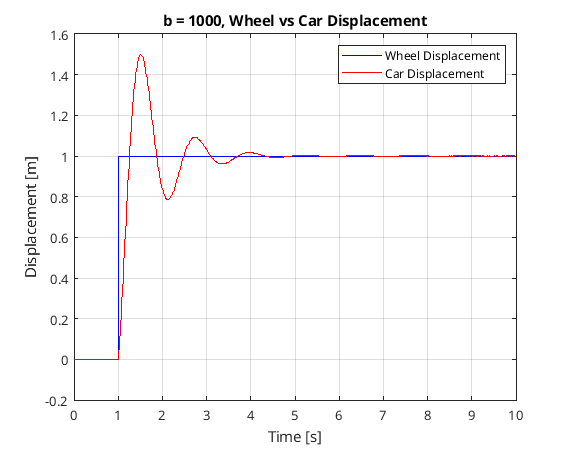
\includegraphics[width=0.75\textwidth]{b1000sim.png}
\end{figure}

At 10,0000 it looks really good actually.
There is a little bump but the output tracks the input pretty closely.
Perhaps this would be worse for a suspension in a way, like too stiff, and you would want the response to take a little bit of time to settle.

\begin{figure}[H]
    \centering
    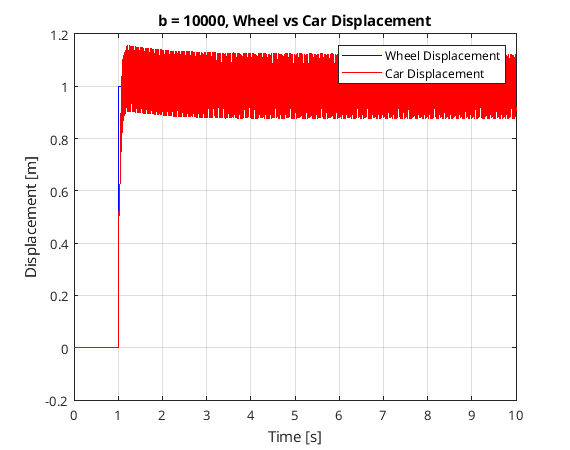
\includegraphics[width=0.75\textwidth]{b10000sim.png}
\end{figure}

Interestingly at 100,000 there is a new, faster oscillation that is introduced.
It's hard to imagine exactly what that would look like or why setting the damping too high would create an oscillatory effect, but interesting.

\begin{figure}[H]
    \centering
    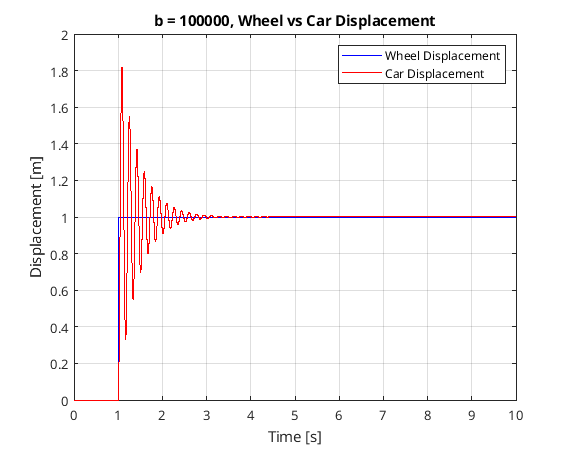
\includegraphics[width=0.75\textwidth]{b100000sim.png}
\end{figure}

\section{}

\textit{
    "Problem 2.7. This is an extension of Problem 2.5, adding active control to a car
    suspension."
}

Problem statement 2.7 from text:

\textit{
    "2.7. Automobile manufacturers are contemplating building active suspension systems. The simplest change is to make shock absorbers with a changeable damping, 
    b($u_1$). It is also possible to make a device to be placed in parallel with the springs that has the ability to supply an equal force, 
    $u_2$, in opposite directions on the wheel axle and the car body.
}
\begin{enumerate}[label=\alph*)]
    \item \textit{Modify the equations of motion in Example 2.2 to include such control inputs.}
    \item \textit{Is the resulting system linear?}
    \item \textit{Is it possible to use the force $u_2$ to completely replace the springs and shock absorber? Is this a good idea?"}
\end{enumerate}

I started by recreating the model using Simulink and adding in the force sources the problem statement describes.
I've put two of them in parallel with each spring and labelled them both $f_1$ because they represent the same input force going up and down into $m_1$ and up into $m_2$.

\begin{figure}[H]
    \centering
    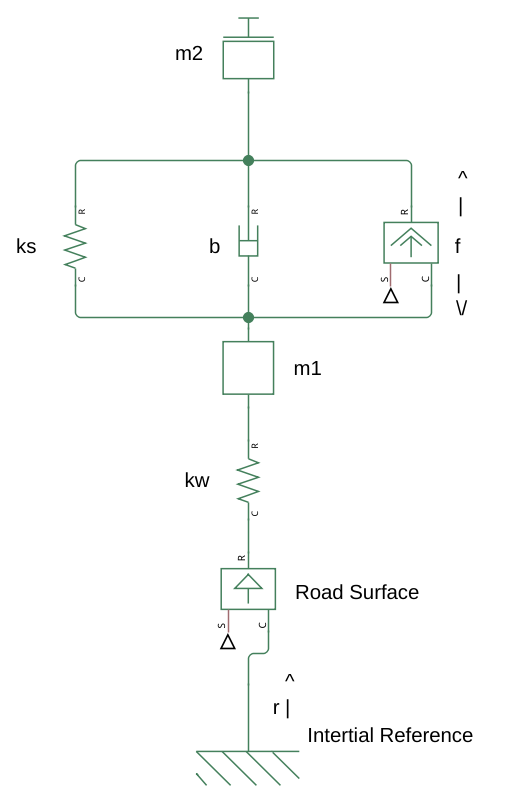
\includegraphics[width=0.5\textwidth]{activeSusModel.png}
\end{figure}

Then I rewrote the state space equations:

\subsection{Identify}
\subsubsection{Input}
\begin{align*}
\text{Wheel Displacement: } & u_1 = r \\
\text{Changeable damping: } & u_2 = b \\
\text{Active suspension: } & u_3 = f
\end{align*}

\subsubsection{Output}
\begin{align*}
\text{Output: } & y = y
\end{align*}

\subsubsection{States}
\begin{align*}
\text{Mass 2: } & x_1 = v_{m_2} = \dot{y} \\
\text{Spring K: } & x_2 = f_{k_s} \\
\text{Mass 1: } & x_3 = v_{m_1} \\
\text{Spring W: } & x_4 = f_{k_w}
\end{align*}

\subsection{Canonical State Variables}
\begin{align*}
x^*_1 &= f_{m_2}, \quad x^*_2 = v_{k_s}, \quad x^*_3 = f_{m_1}, \quad x^*_3 = v_{k_w}
\end{align*}

\subsection{Topology Equations}
\begin{align*}
x^*_1 &= f_{m_2} = -f_{k_s} - f_b - f = -f_{k_s} - bv_b - f = -f_{k_s} - b(v_{m_2} - v_{m_1}) - f = -x_2 - b(x_1 - x_3)  - f \\
x^*_2 &= v_{k_s} = v_{m_2} - v_{m_1} = x_1 - x_3 \\
x^*_3 &= f_{m_1} = -f_{k_w} + f_{k_s} + f_b + f = -x_4 + x_2 + b(x_1 - x_3) + f\\
x^*_4 &= v_{k_w} = v_{m_1} - \dot{r} = x_3 - \dot{r}
\end{align*}

\subsection{Energy Storage Element Equations}
\begin{align*}
x^*_1 &= f_{m_2} = m_2 \dot{v}_{m_2} = m_2 \dot{x}_1 \Rightarrow \dot{x}_1 = \frac{1}{m_2} (x_1^*) = \frac{1}{m_2} (-x_2 - b(x_1-x_3) - f) \\
x^*_2 &= v_{k_s} = \frac{1}{k_s} \dot{f}_{k_s} = \frac{1}{k_s} \dot{x}_2 \Rightarrow \dot{x}_2 = k_s x^*_2 = k_s (x_1 - x_3) \\
x^*_3 &= f_{m_1} = m_1 \dot{v}_{m_1} = m_1 \dot{x}_3 \Rightarrow \dot{x}_3 = \frac{1}{m_1} (x_3^*) = \frac{1}{m_1} (-x_4 + x_2 + b(x_1 - x_3) + f) \\
x^*_4 &= v_{k_w} = \frac{1}{k_w} \dot{f}_{k_w} = \frac{1}{k_w} \dot{x}_4 \Rightarrow \dot{x}_4 = k_w(x^*_4) = k_w (x_3 - \dot{r})
\end{align*}

\subsection{Collect in Matrix Form}

Setting up $b$ as an input creates a nonlinearity here where two variables are being multiplied together.
The input $b$ and the state $x_1$ are being multiplied in the energy storage element equation for $\dot{x_1}$.
I don't think you can and it doesn't really make sense to put the system into matrix form since one of the states is dependent on an input and vice versa.

\subsection*{Replacing Springs and Shock Absorber}

I was having a hard time conceptualizing the last part of the question where you completely replace the spring/damper with just the force actuator so I did some of the state space equations and simulation.

\begin{figure}[H]
    \centering
    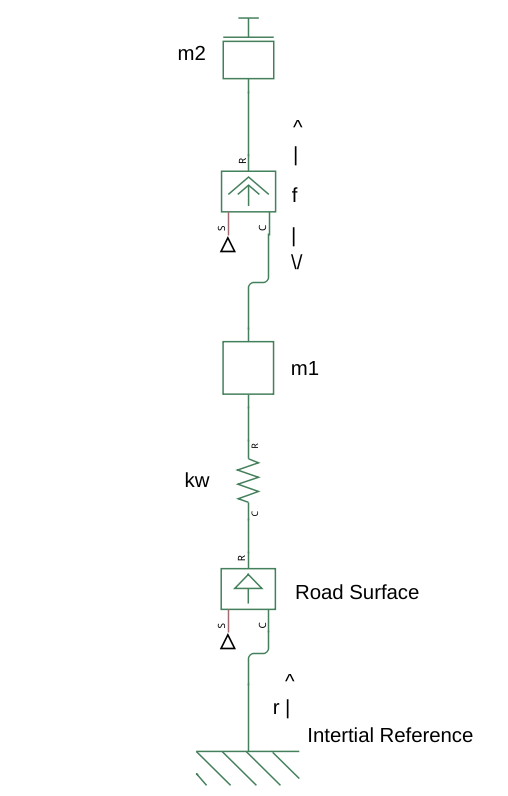
\includegraphics[width=0.5\textwidth]{actSusOnlyModel.png}
\end{figure}

\subsection{Identify}
\subsubsection{Input}
\begin{align*}
\text{Wheel Displacement: } & u_1 = r \\
\text{Active suspension: } & u_2 = f
\end{align*}

\subsubsection{Output}
\begin{align*}
\text{Output: } & y = y
\end{align*}

\subsubsection{States}
\begin{align*}
\text{Mass 2: } & x_1 = v_{m_2} = \dot{y} \\
\text{Mass 1: } & x_2 = v_{m_1} \\
\text{Spring W: } & x_3 = f_{k_w}
\end{align*}

\subsection{Canonical State Variables}
\begin{align*}
x^*_1 &= f_{m_2}, \quad x^*_2 = f_{m_1}, \quad x^*_3 = v_{k_w}
\end{align*}

\subsection{Topology Equations}
\begin{align*}
x^*_1 &= f_{m_2} = -f \\
x^*_2 &= f_{m_1} = -f_{k_w} + f = -x_3 + f \\
x^*_3 &= v_{k_w} = v_{m_1} - \dot{r} = x_2 - \dot{r}
\end{align*}

\subsection{Energy Storage Element Equations}
\begin{align*}
x^*_1 &= f_{m_2} = m_2 \dot{v}_{m_2} = m_2 \dot{x}_1 \Rightarrow \dot{x}_1 = \frac{1}{m_2} (x_1^*) = -\frac{1}{m_2} f \\
x^*_2 &= f_{m_1} = m_1 \dot{v}_{m_1} = m_1 \dot{x}_2 \Rightarrow \dot{x}_2 = \frac{1}{m_1} (x_2^*) = \frac{1}{m_1} (-x_3 + f) \\
x^*_3 &= v_{k_w} = \frac{1}{k_w} \dot{f}_{k_w} = \frac{1}{k_w} \dot{x}_3 \Rightarrow \dot{x}_3 = k_w(x^*_3) = k_w (x_2 - \dot{r})
\end{align*}

\subsection{Collect in Matrix Form}
   
\[
\begin{bmatrix}
\dot{x}_1 \\
\dot{x}_2 \\
\dot{x}_3 
\end{bmatrix}
=
\begin{bmatrix}
0 & 0 & 0 \\
0 & 0 & -\frac{1}{m_1} \\
0 & k_w & 0  
\end{bmatrix}
\begin{bmatrix}
x_1 \\
x_2 \\
x_3 
\end{bmatrix}
+
\begin{bmatrix}
0 & -\frac{1}{m_2}\\
0 & \frac{1}{m_1} \\
-k_w & 0& 
\end{bmatrix}
\begin{bmatrix}
\dot{r} \\
f
\end{bmatrix}
\]

\[
y = 
\begin{bmatrix}
1 & 0 & 0
\end{bmatrix}
\begin{bmatrix}
x_1 \\
x_2 \\
x_3 
\end{bmatrix}
+
\begin{bmatrix}
0
\end{bmatrix}
u
\]

I tried some simulations using the state space model and 'lsim' function in Matlab so I could look at what the states were doing.

\begin{lstlisting}[style=matlabstyle]
A = [0 0 0; 0 0 -1/m1; 0 kw 0]; 
B = [0 -1/m2; 0 1/m1; -kw 0];       
C = [1 0 0];        
D = [0];  
carSusSS = ss(A, B, C, D);

t = 0:0.01:10; 
r = zeros(size(t)); 
r(t >= 1) = 1;
f = zeros(size(t)); 
f(t >= 1) = 100;
% f = 1 * sin(35.6 * 2 * pi * t);
u = [r; f];

[y, t, x] = lsim(carSusSS, u, t);
format longG
disp(eig(A));

% Plot the states
figure;
plot(t, x(:,1), 'b-', t, x(:,2), 'r-', t, r, 'g-');
xlabel('Time [s]');
ylabel('Magnitude');
legend('Car Vertical Velocity (x_1, y)[m/s]', 'Wheel Vertical Velocity (x_2)[m/s]', 'Wheel Vertical Displacement (r)[m]');
title('Simulation of Simplified Suspension System');
grid on;
\end{lstlisting}

I simulated a step f input.

\begin{figure}[H]
    \centering
    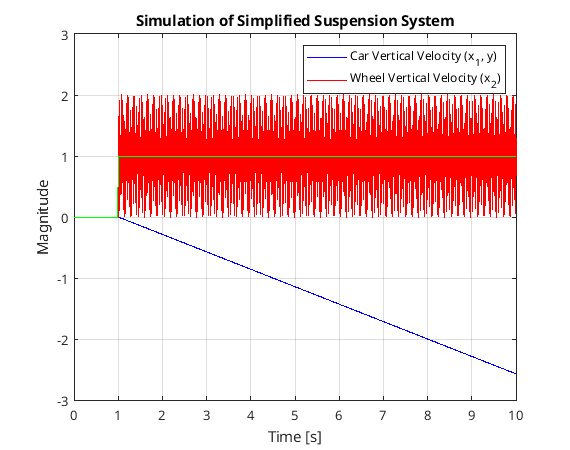
\includegraphics[width=0.5\textwidth]{stepSusOnlySim.png}
\end{figure}

I simulated a sine f input to see what the behavior would look like.

\begin{figure}[H]
    \centering
    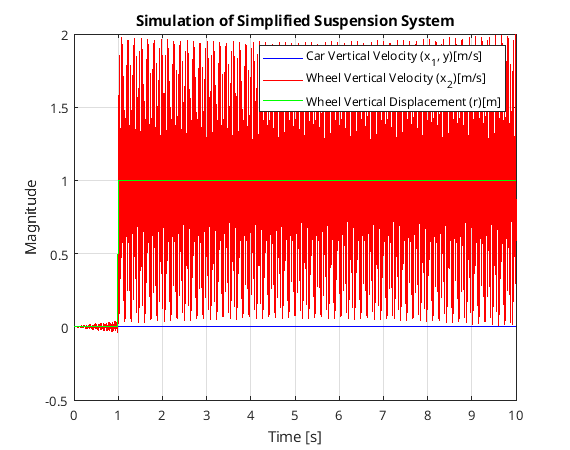
\includegraphics[width=0.5\textwidth]{sinSusOnlySim.png}
\end{figure}

The spring and damper system has this nice behavior where it kind of naturally counteracts and reduces the forces of the wheel movement as it happens, I think in order to get an effect like this you would have to have your force actuator reacting to the changes in input and natural response.
I think if you had some sensors and used a closed loop feedback system you could accomplish the same result which would be an interesting experiment.

\section{}

\textit{
    "Problem 2.22. This is similar to the rigid arm model developed earlier, but with an
    additional flexible mode due to a rotational spring/mass load on the motor. Take the input
    to this system to be $v_a$ [V] and the output to be $\Theta_1$ [rad] (the angle where the flexible
    shaft connects to the motor). Find the eigenvalues of the state space A matrix assuming
    $L_a = 10 [mH]$, $R_a = 1.0 [Ohm]$, $J_1 = 0.1 [kg \cdot m^2]$, $J_2 = 1.0 [kg \cdot m^2]$, $k = 10 [\frac{Nm}{rad}]$,
    $b = 0.01 [\frac{Nms}{rad}]$, $K_t = 1.0 [Nm/A]$, $K_e = 1.0 [\frac{Vs}{rad}]$, $B = 0.01 [\frac{Nms}{rad}]$. What partial
    fraction terms do you expect in the system response to a step input at $v_a$?"
}

Problem Statement 2.22:

\textit{
    "2.22. A very typical problem of electromechanical position control is an electric motor driving a load that has one dominant vibration mode. The problem arises in computer-disk-head control, reel-to-reel tape drives, and many other applications. A schematic diagram is sketched in Fig. 2.57. The motor has an electrical constant 
    $K_e$, a torque constant 
    $K_t$, an armature inductance 
    $L_a$, and a resistance 
    $R_a$. The rotor has an inertia 
    $J_1$ and a viscous friction $B$. The load has an inertia 
    $J_2$. The two inertias are connected by a shaft with a spring constant $k$ and an equivalent viscous damping $b$. Write the equations of motion."
}

\begin{figure}[H]
    \centering
    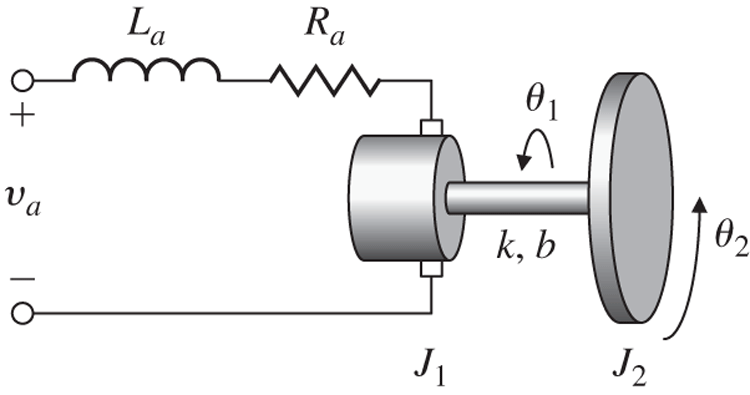
\includegraphics[width=0.75\textwidth]{fig27.png}
\end{figure}

\subsection{Identify}
\subsubsection{Inputs:}
    \[
    u = V_a
    \]

 subsubsection{Outputs:}
    \[
    y = \theta_1
    \]

 subsubsection{States:}
    \[
    L_a : x_1 = i_a
    \]
    \[
    \text{shaft:} \ x_2 = \theta_1 = y_1, \ x_3 = \dot{\theta}_1
    \]
    \[
    \text{load:} \ x_4 = \theta_2, \ x_5 = \dot{\theta}_2
    \]

\subsection{Complementary State Variables}
\[
x^*_1 = V_{La}, \ x^*_3 = \tau_1, \ x^*_5 = \tau_2
\]

\subsection{Topology Equations}
\[
x^*_1 = V_a - R_a i_a - K_e \dot{\theta}_1
\]
\[
= V_a - R_a x_1 - K_e x_3
\]

\[
x^*_3 = \tau_1 = K_t i_a - B \dot{\theta}_1 - k(\theta_1 - \theta_2) - b(\dot{\theta}_1 - \dot{\theta}_2)
\]
\[
= K_t x_1 - B x_3 - k(x_2 - x_4) - b(x_3 - x_5)
\]

\[
x^*_5 = \tau_2 = k(\theta_1 - \theta_2) + b(\dot{\theta}_1 - \dot{\theta}_2)
\]
\[
= k(x_2 - x_4) + b(x_3 - x_5)
\]

\subsection{Energy Storage Element Equations}
\[
x_1^* = V_{L_a} = L_a \dot{i}_a = L_a \dot{x}_1 \Rightarrow \dot{x}_1 = \frac{1}{L_a} (V_a - R_a x_1 - K_e x_3)
\]

\[
x_3^* = \tau_1 = J_1 \ddot{\theta}_1 = J_1 \dot{x}_3 \Rightarrow \dot{x}_3 = \frac{1}{J_1} \left( K_t x_1 - B x_3 - k(x_2 - x_4) - b(x_3 - x_5) \right)
\]

\[
x_5^* = \tau_2 = J_2 \ddot{\theta}_2 = J_2 \dot{x}_5 \Rightarrow \dot{x}_5 = \frac{1}{J_2} \left( k(x_2 - x_4) + b(x_3 - x_5) \right)
\]

\subsection{Matrix Form}
\[
\begin{bmatrix}
\dot{x}_1 \\
\dot{x}_2 \\
\dot{x}_3 \\
\dot{x}_4 \\
\dot{x}_5
\end{bmatrix}
=
\begin{bmatrix}
-\frac{R_a}{L_a} & 0 & -\frac{K_e}{L_a} & 0 & 0 \\
0 & 0 & 1 & 0 & 0 \\
\frac{K_t}{J_1} & -\frac{k}{J_1} & \frac{-B-b}{J_1} & \frac{k}{J_1} & \frac{b}{J_1} \\
0 & 0 & 0 & 0 & 1 \\
0 & \frac{k}{J_2} & \frac{b}{J_2} & -\frac{k}{J_2} & -\frac{b}{J_2}
\end{bmatrix}
\begin{bmatrix}
x_1 \\
x_2 \\
x_3 \\
x_4 \\
x_5
\end{bmatrix}
+
\begin{bmatrix}
\frac{1}{L_a} \\
0 \\
0 \\
0 \\
0
\end{bmatrix}
u
\]

\[
y =
\begin{bmatrix}
0 & 1 & 0 & 0 & 0
\end{bmatrix}
\begin{bmatrix}
x_1 \\
x_2 \\
x_3 \\
x_4 \\
x_5
\end{bmatrix}
+
\begin{bmatrix}
0
\end{bmatrix}
u
\]

\subsection*{Eigenvalues}

I got the Eigenvalues by plugging the state space model into Matlab and using the 'eig' function:

\begin{lstlisting}[style=matlabstyle]
La = 0.010; % [H]
Ra = 1.0; % [Ohm]
J1 = 0.1; % [kg m^2]
J2 = 1.0; % [kg m^2]
k = 10; % [Nm/rad]
b = 0.01; % [Nms/rad]
Kt = 1.0; % [Nm/A]
Ke = 1.0; % [Vs/rad]
B = 0.01; % [Nms/rad]

A = [-Ra/La 0 -Ke/La 0 0; 0 0 1 0 0; Kt/J1 -k/J1 (-B-b)/J1 k/J1 b/J1; 0 0 0 0 1; 0 k/J2 b/J2 -k/J2 -b/J2]; 
B = [1/La; 0; 0; 0; 0];       
C = [0 1 0 0 0];        
D = [0];  

rotorSS = ss(A, B, C, D);

disp(eig(rotorSS));    
\end{lstlisting}

The results were:

\[
\begin{aligned}
&\lambda_1 = -88.8624852873471 + 0i \\
&\lambda_2 = -5.16707795875504 + 9.24455182135315i \\
&\lambda_3 = -5.16707795875504 - 9.24455182135315i \\
&\lambda_4 = -1.01335879514286 + 0i \\
&\lambda_5 = -2.10746545361914 \times 10^{-16} + 0i
\end{aligned}
\]

I would expect a term that would essentially just be 0/s for the step input, I would expect a term that would be very close to something over s-0 for that fifth Eigenvalue that is very close to 0, I would expect there to be a couple terms like something over $(s-\lambda_2)^2$ for the complex conjugate terms and one $(s-\lambda_1)$ for the negative real Eigenvalue.

$\lambda_5$ implies that the system is close to not be stable but all of the natural response would eventually disappear.

\begin{figure}[H]
    \centering
    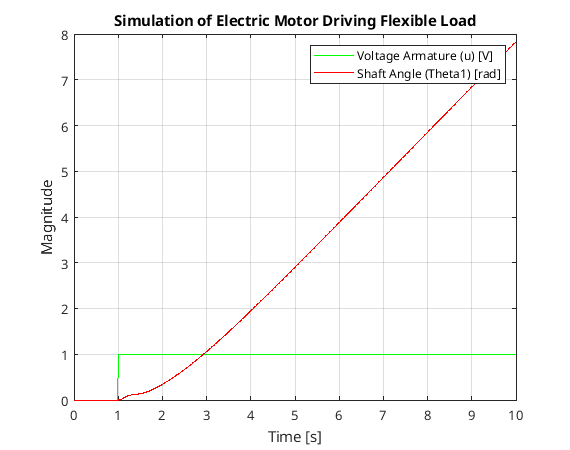
\includegraphics[width=0.75\textwidth]{rotorSim.png}
\end{figure}

\end{document}